\chapter{Diseño y desarrollo de la aplicación\label{sec:disenho}}

En este trabajo fin de Máster, se ha decidido comparar los sistemas de captura de tráfico \textit{PF\_RING}, \textit{HPCAP}, \textit{Intel \gls{dpdk}} y el driver \gls{vanilla} de Intel (\textit{ixgbe}).
De cara a comparar estos sistemas es necesario disponer de algún tipo de herramienta que haga uso de susodicho sistema para medir de forma precisa los paquetes recibidos y perdidos sin ningún tipo de proceso.
Mediante esta métrica, es posible determinar el comportamiento de un motor de captura en un entorno muy favorable, proporcionando una cota de rendimiento o fiabilidad del sistema máxima. 
Por otro lado, es importante evaluar la capacidad de estos motores para trabajar en conjunto con otros elementos. Dado que resulta interesante almacenar el tráfico capturado para realizar posteriores análisis, se ha decidido evaluar la capacidad de estos motores almacenando a tasa de linea en disco.

No obstante, \textit{Intel \gls{dpdk}} no ofrece una herramienta simple para medir la tasa de recepción en una \gls{nic}, y al igual que \textit{PF\_RING}, no existe ninguna aplicación que utilicen estos motores de captura y sean capaces de almacenar a disco a tasa de linea (o al menos hasta donde llega mi conocimiento). Para poder desarrollar y diseñar estos sistemas de captura y almacenado, es de vital importancia conocer cuales serán los escenarios en los que se podrían utilizar.

\lsection{Escenarios de captura}

Cuando se piensa en un entorno de captura y almacenamiento (y en principio de procesado y análisis) de red, surge de forma natural el concepto de \gls{mpasiva}. Es extraño imaginar en un contexto real a un único servidor sirviendo peticiones a 10 o incluso a más~Gbps. No obstante, parece razonable pensar que varios cientos o incluso miles de nodos se encuentren atendiendo miles o millones de peticiones a tasas mas bajas que, por otro lado, agregadas pueden llegar a superar fácilmente los 10 o incluso 40~Gbps en ciertas compañías.

Bajo esta clásica idea, podemos imaginarnos un sistema (Ver Fig.~\ref{fig:dis:arq}) en el que una gran cantidad de máquinas se encuentran conectadas entre sí mediante uno o varios switches o routers. Dado que estos sistemas suelen acceder de una forma u otra a Internet, no es de extrañarse que en algún punto de la red se encuentre al menos una salida de alta velocidad hacia el resto de Internet. Dado que este enlace supone una vulnerabilidad para la red, suele encontrarse protegido por un cortafuegos. No obstante, una habilidoso atacante podría llegar a franquear el cortafuegos y entrar de una forma u otra en la red.
Dado que trabajar con una elevada cantidad de dispositivos en la red, causa un inevitable aumento en la probabilidad de fallo o ataque en alguno de ellos, parece sensato disponer de algún sistema de monitorización que al menos vigile que la red se encuentra en un estado adecuado. 

%Arquitectura de captura tradicional

\begin{figure}[!th]
\centering
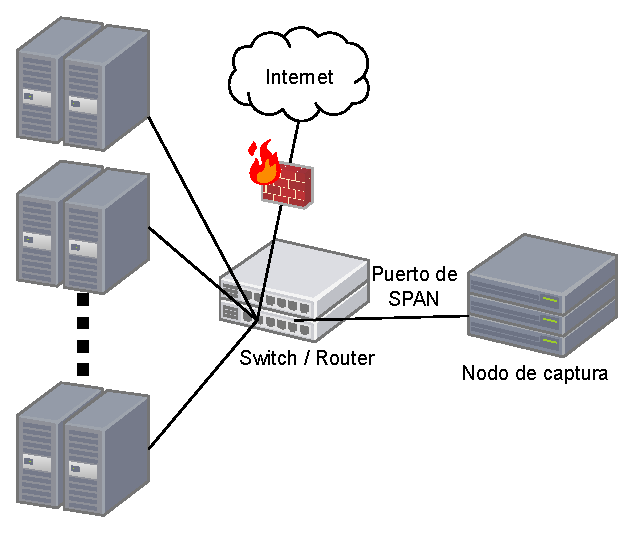
\includegraphics[scale=.7]{arq}
\caption{Arquitectura de captura tradicional}
\label{fig:dis:arq}
\end{figure}

No obstante, añadir un nuevo equipo a una red, suele suponer la implantación de un equipo grande (4\gls{U}) y de elevado coste dentro del \gls{cpd} en donde se encuentran los equipos y la red que desean ser monitorizados. También hay que tener en cuenta, que añadir un nuevo equipo supone una serie de riesgos de seguridad para la empresa propietaria de la red y de los equipos y que en ciertos casos, puede no ser asumible.

Dejando estos problemas de lado, es importante tener en cuenta que esta visión de como funciona un~\gls{cpd} y por ende, esta definición de la arquitectura de red es muy diferente a la visión tradicional. Actualmente, y desde la popularización del \gls{cloud}, resulta difícil de imaginar un dispositivo dedicado en exclusiva a una única tarea. De forma habitual, una aplicación (como puede ser un servidor web o una base de datos) no explota completamente los recursos de la máquina en la que se ejecuta. Por este motivo, los \glspl{cpd} actuales(Ver Fig.~\ref{fig:dis:arqvm}) disponen de grandes y potentes máquinas que permiten ejecutar multitud de pequeñas máquinas virtuales dedicadas a tareas muy concretas. Esta división en pequeñas tareas o servicios viene de la mano con el auge de los sistemas distribuidos (como Hadoop~\cite{hadoop,hadoop-definitive-guide}), cuyo objetivo es la resolución de un gran problema a base de fragmentarlo en pequeños trozos y procesarlos en paralelo.

%Arquitectura en un sistema virtual

\begin{figure}[!th]
\centering
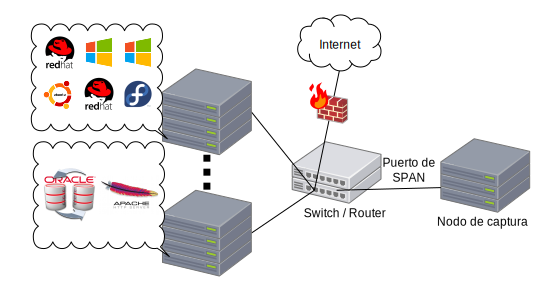
\includegraphics[scale=.7]{arqvm}
\caption{Arquitectura de captura en un sistema con virtualización}
\label{fig:dis:arqvm}
\end{figure}

La aparición de la virtualización, al igual que aumenta la rentabilidad de los servidores, hace surgir nuevos problemas que en un escenario tradicional no se presentaban. Dentro de un único servidor, están presentes varios sistemas operativos, así como sus respectivas aplicaciones. Comunicar las diferentes máquinas virtuales con el exterior supone una decisión crítica a la hora de definir cada una de las \gls{vm}.
Virtualizar las tarjetas de red con \textit{Passthrough} permite explotar las tarjetas de red al máximo, por otro lado, esto requeriría una tarjeta de red completa por cada una de las máquinas virtuales que fuesen a ejecutarse en la máquina física, además de un aumento en el número de cables y en la capacidad de los switches para interconectarlas.

Dada que una de las bases de las máquinas virtuales es la compartición de recursos, estas máquinas virtuales suelen utilizar virtualizaciones completas de las tarjetas de red, para virtualizaciones de las mismas, o en su defecto, \glspl{nfv}. Esta compartición de las interfaces de red, provoca que la tarjeta de red actué como un switch virtual entre las diferentes \glspl{vm} que la comparten. Aunque esto, a priori, no parece suponer un problema, hay que tener en cuenta que el objetivo es monitorizar el tráfico de una determinada red. Todo el tráfico interno entre máquinas virtuales no llega nunca a salir al nodo de captura de la figura~\ref{fig:dis:arqvm}, perdiéndose información potencialmente relevante para la motorización de la red.

%Arquitectura en un sistema completo virtual

\begin{figure}[!th]
\centering
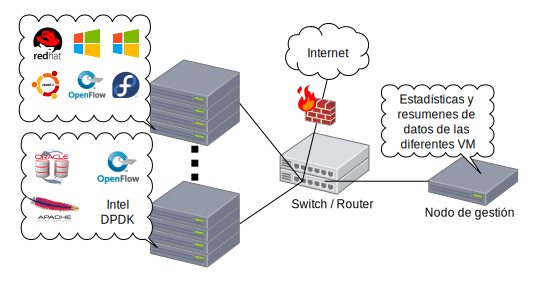
\includegraphics[scale=.7]{arqfullvm}
\caption{Arquitectura de un sistema de captura completamente virtualizado}
\label{fig:dis:arqfullvm}
\end{figure}

La única forma de solventar este problema, supone la inserción de un elemento en las máquinas anfitrionas que monitorice dicho tráfico. La forma mas simple de hacerlo, radica en insertar una máquina virtual en cada máquina física, de forma que recoja y procese el tráfico del resto de \glspl{vm} de su anfitriona.
En caso de lograr posicionar una \gls{vm} en cada nodo físico a monitorizar, la necesidad de disponer de una máquina de captura desaparece completamente. No obstante, al tener un conjunto de \glspl{vm} monitorizando fragmentos de la red, aparece el concepto de agente (o nodo) de gestión de monitorización. Este nodo, que bien puede ser un elemento físico u otra \gls{vm}, se encargaría de recoger la información capturada y procesada en las distintas \glspl{vm} de monitorización y centralizar los resultados bajo un único punto de acceso. La figura~\ref{fig:dis:arqfullvm} muestra una representación gráfica del escenario previamente descrito. Aunque está presente el elemento \textit{OpenFlow} en el dibujo, podría ser sustituido por cualquier otro agente de monitorización y captura de tráfico.

\lsection{Sistema de captura diseñado}

A raíz de los escenarios descritos previamente, es posible definir los requisitos que requiere nuestra aplicación de captura de red.
En el peor de los casos, esta aplicación debe ser capaz de capturar y almacenar el tráfico a tasa de linea, es decir: 10~Gbps.
Del mismo modo, la aplicación debe ser capaz de trabajar tanto en entornos físicos como en entornos virtuales (Ya sea mediante dispositivos \gls{virtio}, como \glspl{nfv}).
Para lograrlo, dicha herramienta, debe utilizar la API de Intel~\gls{dpdk} para lograr interoperatividad con diferentes tarjetas de red.

%El funcionamiento interno de esta API es muy conocido y ha sido estudiado previamente en trabajos anteriores~\cite{rleira2013TFG,dpdk:Leir1306}.

Para crear una aplicación con Intel~\gls{dpdk}, hay que tener en cuenta su diseño orientado a la construcción de pipelines y explotación de paralelismo. El funcionamiento de comunicación entre diferentes elementos en una aplicación \gls{dpdk} se basa en la utilización de anillos. Cada anillo, está diseñado como una cola circular que almacena punteros a descriptores de paquetes. Cada descriptor de paquete, a su vez almacena el tamaño del paquete y un puntero al contenido del mismo. De esta forma, al mover un paquete entre diferentes hilos, no es necesario copiar el contenido del paquete, optimizándose los accesos y escrituras de memoria.

Con el objetivo inicial en mente, de evaluar \gls{dpdk} en el mejor caso posible (sin procesamiento), se ha desarrollado una aplicación con único hilo. Dicha aplicación captura todos y cada uno de los paquetes y libera los recursos asociados tan pronto es posible. Tras haber recibido un determinado número de paquetes, imprime por pantalla uno valor estimado de ancho de banda, así como cantidad de paquetes recibidos y perdidos (ya sea por errores en los paquetes u otros efectos). Dado que el funcionamiento en detalle de la API es muy conocido~\cite{dpdk2015} y ha sido estudiado previamente en trabajos anteriores~\cite{rleira2013TFG,dpdk:Leir1306}, considero que no es necesario entrar en detalles implementativos de la aplicación. En la figura~\ref{fig:dis:dpdktest} se muestra una representación gráfica del flujo de datos en la aplicación, mientras que en~\cite{dpdkspeedometer} puede descargarse esta aplicación.

\begin{figure}[!th]
\centering
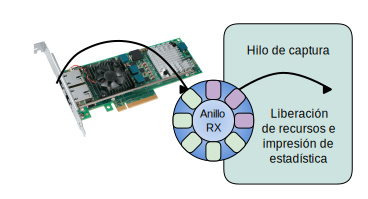
\includegraphics[scale=.7]{dpdktest}
\caption{Arquitectura de un sistema de captura con DPDK}
\label{fig:dis:dpdktest}
\end{figure}


\begin{figure}[!th]
\centering
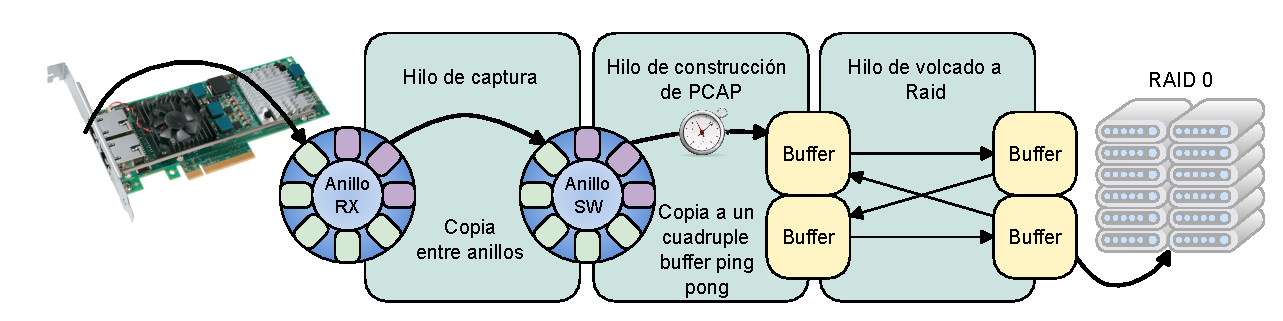
\includegraphics[scale=.7]{dpdkdd}
\caption{Arquitectura de un sistema de captura y almacenamiento con DPDK}
\label{fig:dis:dpdkdd}
\end{figure}

